\subsection{ScriptableObject (Bogna Lew)}\label{ss:so}
Silnik Unity umożliwia użytkownikom tworzenie klas typu \texttt{ScriptableObject}. Jest to struktura danych, która pozwala na
tworzenie wielu instancji klasy bez konieczności kopiowania danych. Poszczególne instancje współdzielą informacje, dzięki
czemu możliwe jest znaczące zoptymalizowanie użycia pamięci.

Do podstawowych zalet ScriptableObject należy możliwość wykorzystania go do tworzenia zasobów, które można by wykorzystać
w trakcie gry. Dzięki temu w prosty sposób można utworzyć szablony dla obiektów takich jak budowle, bronie i inne
przedmioty, które następnie można użyć do utworzenia jego instancji podczas rozgrywki.

\begin{figure}[h!]
    \centering
    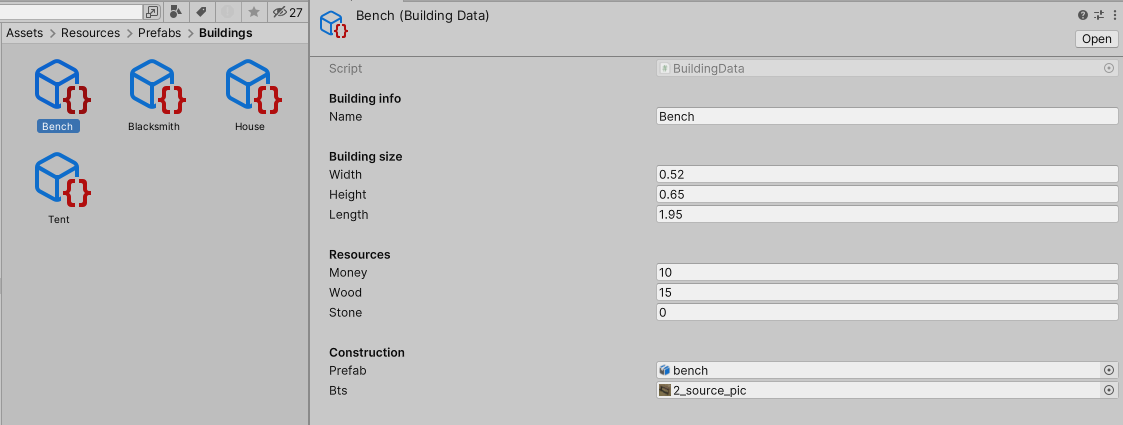
\includegraphics[width=0.9\textwidth]{images/scriptableobjects.jpg}
    \caption{Przykład zasobów typu \texttt{ScriptableObject}.}
\end{figure}
\FloatBarrier
